\documentclass[11pt]{article}
\usepackage[a4paper]{geometry}
\usepackage{polski}
\usepackage{hyperref}
\usepackage[utf8]{inputenc}
\usepackage[table,xcdraw]{xcolor}
\usepackage{graphicx}[demo]
\usepackage{tikz}
\usepackage{float}
\usepackage[usestackEOL]{stackengine} 
\usepackage{caption}
\usetikzlibrary{shapes,arrows,chains}
\usetikzlibrary[calc]
\linespread{1.3}
\usepackage{listings}
\usepackage{indentfirst}

\begin{document}
\begin{titlepage}
\newcommand{\HRule}{\rule{\linewidth}{0.5mm}} % Defines a new command for the horizontal lines, change thickness here
\center % Center everything on the page
%	LOGO SECTION

\includegraphics[scale = 0.21]{pwr-logo.png}\\[2cm]
%	HEADING SECTIONS
\textsc{\Large Programowaniie Obiektowe}\\[0.5cm] 
\textsc{\large projekt wtorek 17:05}\\[0.5cm]
%	TITLE SECTION
\HRule \\[0.4cm]
{ \huge \bfseries Symulacja Domu Towarowego
}\\[0.4cm] 
\HRule \\[0.8cm]
%	AUTHORS SECTION
\begin{minipage}{0.5\textwidth}
\begin{flushleft} \large
\emph{Autor:}\\
\textbf{Gabriel \textsc{Malanowski} 281081} \\
Kamil \textsc{Kondrat} 281177 \\

\end{flushleft}
\end{minipage}
~
\begin{minipage}{0.4\textwidth}
\begin{flushright} \large
\emph{Prowadzący:} \\
mgr inż. Tobiasz \textsc{Puślecki} % supervisor
\end{flushright}
\end{minipage}\\[5cm]

\vfill % Fill the rest of the page with whitespace
\end{titlepage}
\newgeometry{bmargin=2cm, tmargin=2cm, lmargin=2cm, rmargin=2cm}
\newpage




\section{Wstęp}

Projekt Symulacja Domu Towarowego to system wspomagający zarządzanie magazynem, który umożliwia symulowanie i optymalizowanie procesów magazynowych. Dzięki niemu użytkownicy mogą modelować różne scenariusze, analizować wyniki oraz podejmować decyzje w czasie rzeczywistym. Projekt integruje algorytmy symulacyjne z interaktywnym interfejsem użytkownika, co pozwala na dynamiczne monitorowanie stanu magazynu oraz szybką reakcję na zmiany w otoczeniu biznesowym. Główne cechy projektu obejmują definiowanie magazynów, produktów, atrybutów, symulację działania magazynu w pętli czasowej, generowanie zdarzeń, interwencję użytkownika oraz generowanie raportów z wynikami symulacji. Celem projektu jest dostarczenie narzędzia wspomagającego efektywne zarządzanie magazynem, które pozwoli firmom na zwiększenie efektywności operacyjnej i maksymalizację zysków.

\section{Opis}

\subsection{Ogólny opis symulacji}
Użytkownik podaje informacje o magazynach oraz produktach w magazynie. Każdy obiekt ma swoje atrybuty, takie jak pojemność magazynu, cena produktu. Symulacja działa w pętli czasowej, gdzie każdy cykl reprezentuje jednostkę czasu (np. godzinę, dzień). W każdym cyklu, symulacja sprawdza stan magazynu i podejmuje decyzje na podstawie zdefiniowanych reguł. Zdarzenia takie jak przyjęcie nowego towaru, sprzedaż produktu, lub zmiana zapotrzebowania są generowane losowo lub według określonego harmonogramu. Symulacja reaguje na te zdarzenia, aktualizując stan magazynu i inne powiązane obiekty. Na podstawie stanu magazynu i nadchodzących zdarzeń, symulacja podejmuje decyzje, takie jak zamówienie nowego towaru, przesunięcie zasobów, czy wysłanie powiadomień do administratorów. Wszystkie działania i zmiany są rejestrowane w systemie, co pozwala na analizę wyników symulacji i optymalizację procesów magazynowych. Użytkownik może interweniować w symulację, wprowadzając zmiany w strategii zarządzania magazynem lub reagując na generowane zdarzenia.
Na koniec symulacji, użytkownik otrzymuje raport z wynikami, takimi jak koszty operacyjne czy zysk netto.

\subsection{Diagram klas}

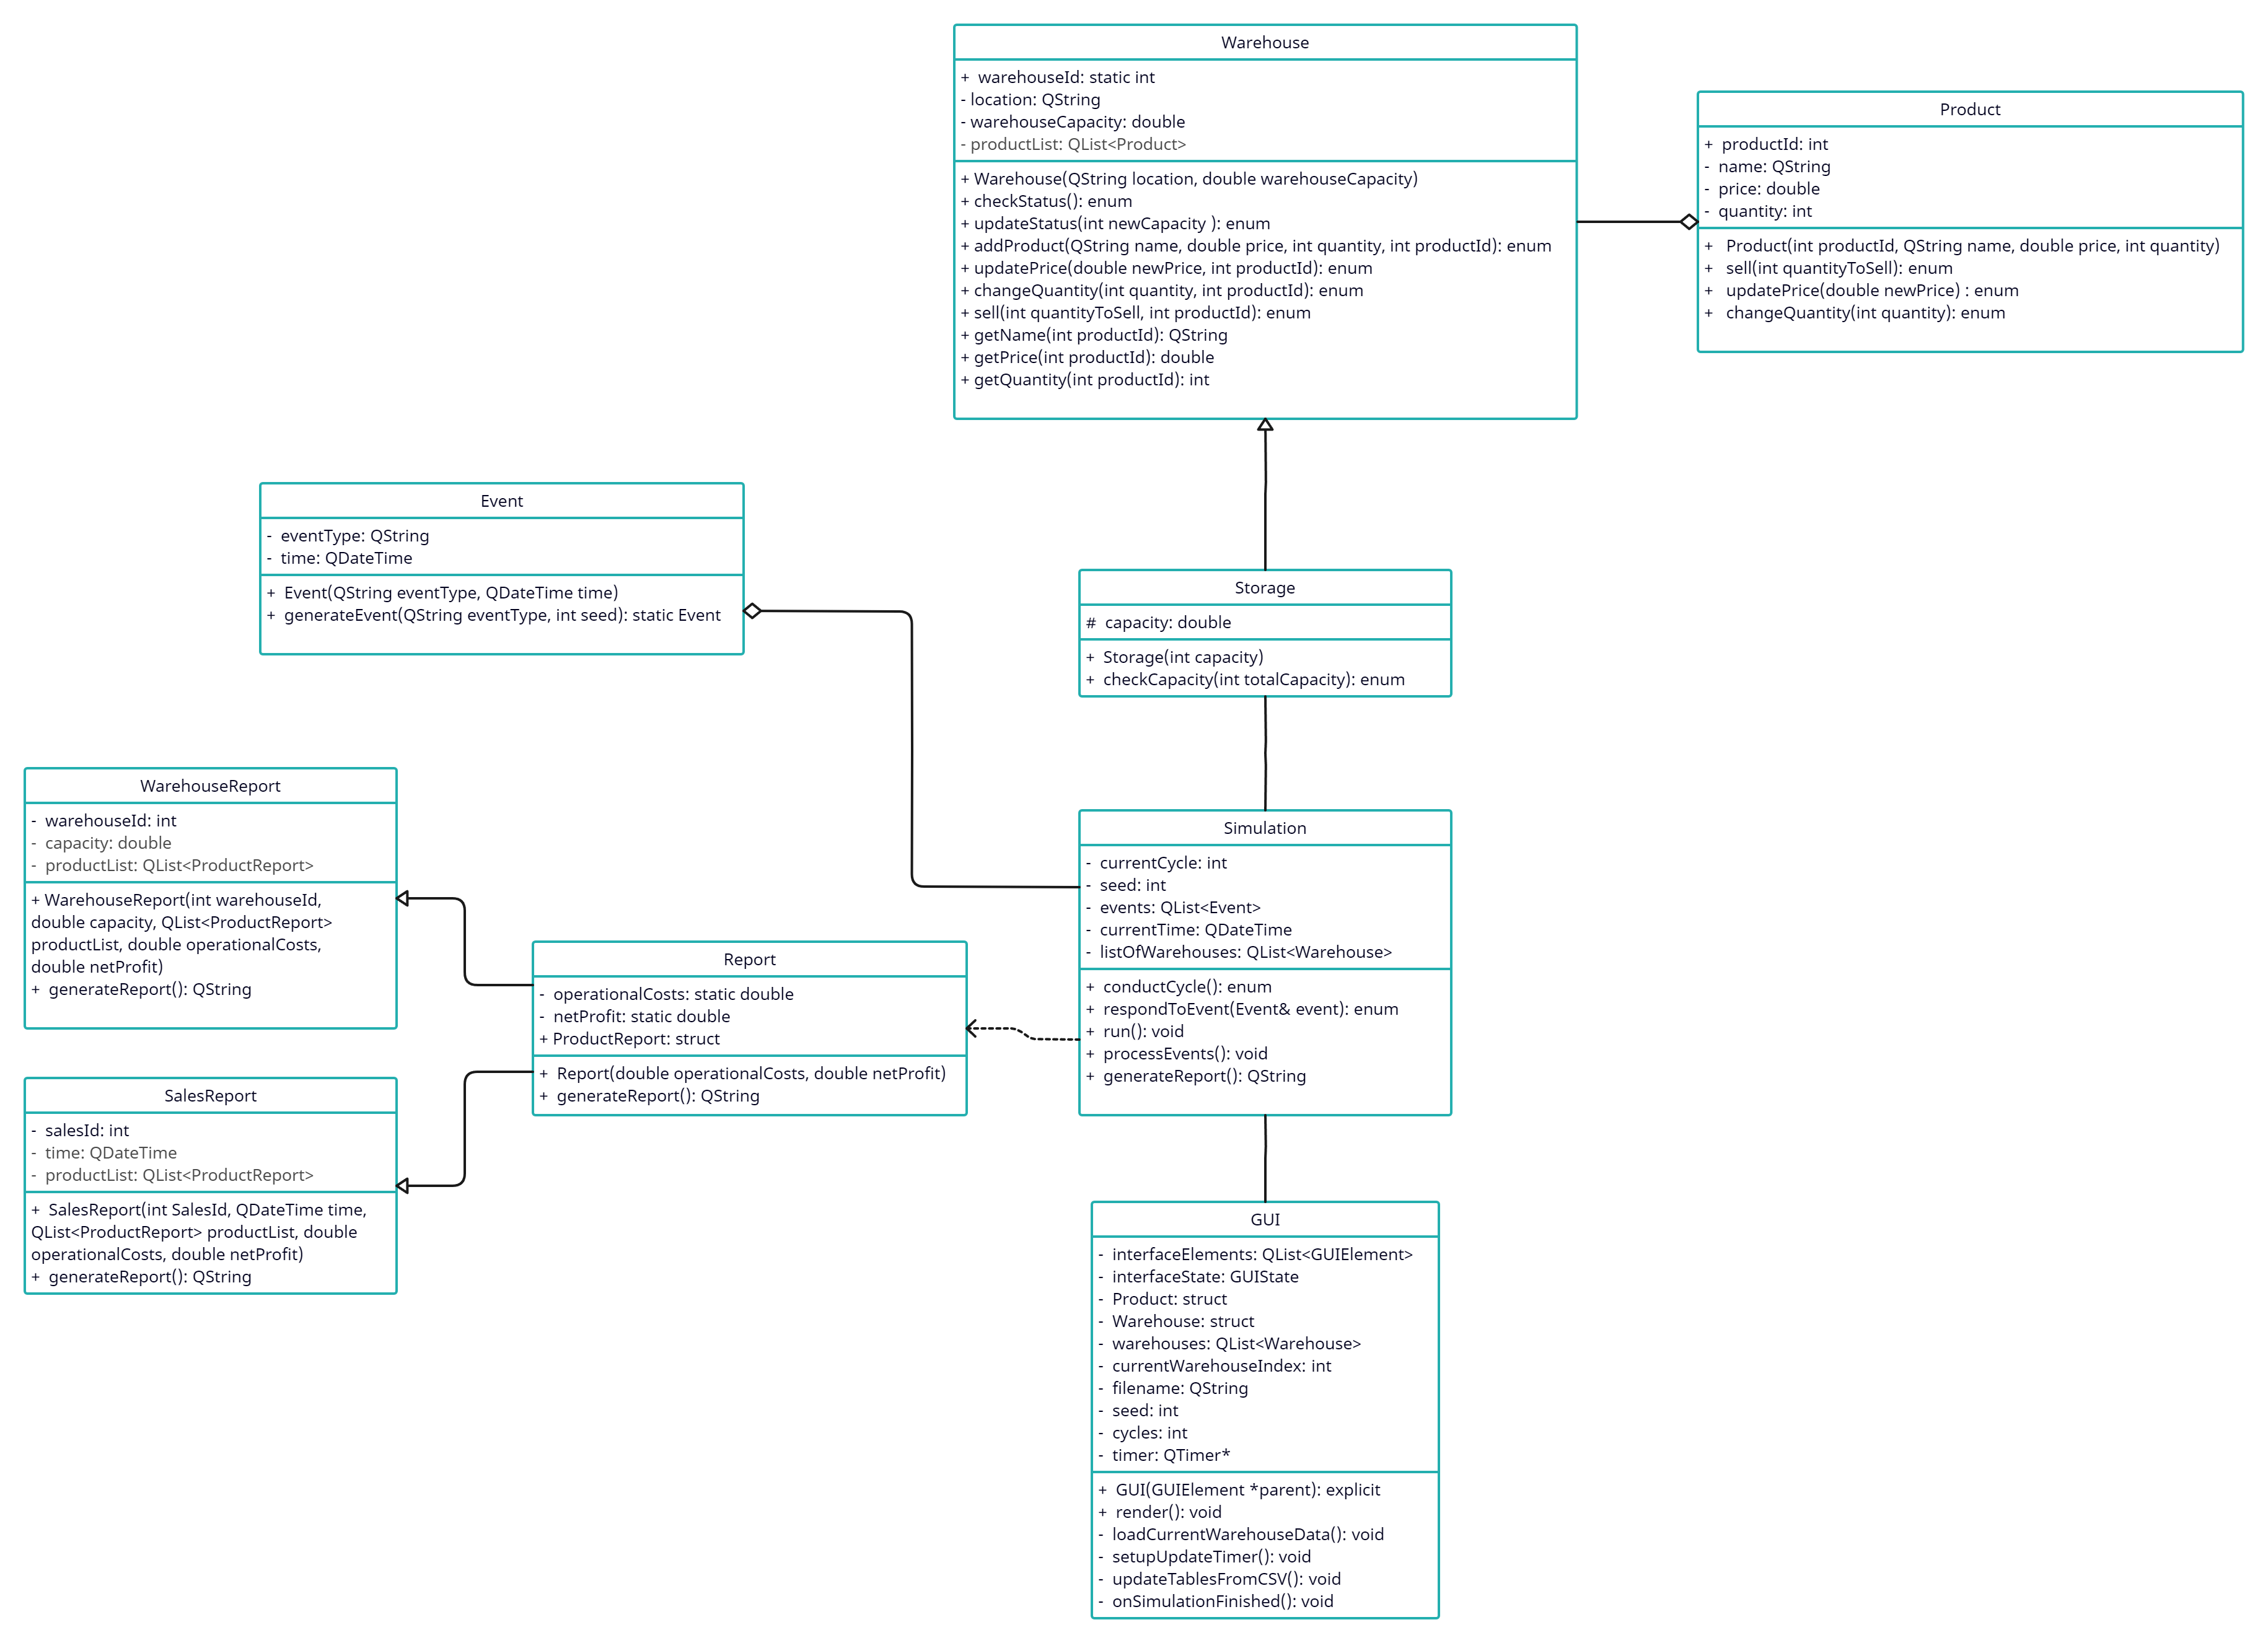
\includegraphics[scale=0.15]{Diagram klas.png}

Opis diagramu klas dla symulacji domu towarowego w języku C++, który spełnia wymienione warunki:

\begin{enumerate}

    \item Klasa \textbf{Simulation} :
    \begin{itemize}
        \item \textbf{Atrybuty:} currentCycle, events, currentTime, eventAgenda, listOfWarehouses.
        \item \textbf{Metody:} conductCycle(), respondToEvent(), run(), processEvents(), generateReport().
    \end{itemize}

    \item Klasa \textbf{Storage} :
    \begin{itemize}
        \item \textbf{Atrybuty:} capacity.
        \item \textbf{Metody:} checkCapacity().
    \end{itemize}

    \item Klasa \textbf{Warehouse} :
    \begin{itemize}
        \item \textbf{Atrybuty:} warehouseId, location, capacity, productList.
        \item \textbf{Metody:} checkStatus(), updateStatus(double newCapacity).
    \end{itemize}

    \item Klasa \textbf{Product} :
    \begin{itemize}
        \item \textbf{Atrybuty:} productId, name, price, quantity.
        \item \textbf{Metody:} sell(int quantityToSell), updatePrice(double newPrice)
        changeQuantity(int quantity).
    \end{itemize}

    \item Klasa \textbf{Event} :
    \begin{itemize}
        \item \textbf{Atrybuty:} eventType, time.
        \item \textbf{Metody:} generateEvent().
    \end{itemize}

    \item Klasa \textbf{Report} :
    \begin{itemize}
        \item \textbf{Atrybuty:} operationalCosts, netProfit.
        \item \textbf{Metody:} generateReport().
    \end{itemize}

    \item Klasa \textbf{WarehouseReport} :
    \begin{itemize}
        \item \textbf{Atrybuty:} warehouseId, capacity, productList.
        \item \textbf{Metody:} generateReport().
    \end{itemize}

    \item Klasa \textbf{SalesReport} :
    \begin{itemize}
        \item \textbf{Atrybuty:} salesId, time, productList.
        \item \textbf{Metody:} generateReport().
    \end{itemize}

\item Klasa \textbf{GUI} :
    \begin{itemize}
        \item \textbf{Atrybuty:} interfaceElements, interfaceState.
        \item \textbf{Metody:} render(), updateGUI(const GUIEvent\& event), handleEvents(const GUIEvent\& event).
    \end{itemize}
    
\end{enumerate}


\textbf{Hermetyzacja} jest zastosowana poprzez ustawienie atrybutów jako prywatnych (\textit{private}) i dostęp do nich poprzez publiczne metody (\textit{public}).
\vspace{1pt}

\textbf{Dziedziczenie} jest reprezentowane przez klasę \textit{Warehouse}, która dziedziczy po klasie \textit{Storage}.
\vspace{1pt}

\textbf{Kompozycja} występuje, gdy \textit{Simulation} zawiera obiekty \textit{Warehouse}, które z kolei zawierają obiekty \textit{Product}..
\vspace{1pt}

\textbf{Agregacja} jest zastosowana w klasie \textit{Simulation} dla klasy \textit{Event}.
\vspace{1pt}

\textbf{Polimorfizm} może być reprezentowany przez różne typy zdarzeń, które są obsługiwane przez metodę \textit{generateReport()} w klasie \textit{Report}. Każde zdarzenie może mieć inną implementację tej metody, w zależności od jego typu.

\newpage

\subsection{Diagram obiektów}

\includegraphics[scale = 0.14]{obiektów.png}

Opis diagramu obiektów dla przykładowej symulacji domu towarowego w języku C++.

\begin{enumerate}

\item Obiekty klasy \textbf{Simulation}
\begin{itemize}
    \item \textbf{simulation}: \{ currentCycle: 5, events: [event1, event2], currentTime: "2023-04-05T14:00:00Z", eventAgenda: "Sale", listOfWarehouses: [warehouse1, warehouse2] \}
\end{itemize}

\item Obiekty klasy \textbf{Storage}
\begin{itemize}
    \item \textbf{storage1}: \{ capacity: 1000 \}
    \item \textbf{storage2}: \{ capacity: 500 \}
\end{itemize}

\item Obiekty klasy \textbf{Warehouse}
\begin{itemize}
    \item \textbf{warehouse1}: \{ warehouseId: 1, location: "Warszawa", capacity: 1000, productList: [product1, product2] \}
    \item \textbf{storage2}: \{ warehouseId: 2, location: "Kraków", capacity: 500, productList: [product3, product4] \}
\end{itemize}

\item Obiekty klasy \textbf{Product}
\begin{itemize}
    \item \textbf{product1}: \{ productId: 101, name: "Laptop", price: 3000, quantity: 50 \}
    \item \textbf{product2}: \{ productId: 102, name: "Phone", price: 2000, quantity: 100 \}
    \item \textbf{product3}: \{ productId: 103, name: "Tablet", price: 1500, quantity: 30 \}
    \item \textbf{product4}: \{ productId: 104, name: "Headphones", price: 300, quantity: 200 \}
\end{itemize}

\item Obiekty klasy \textbf{Event}
\begin{itemize}
    \item \textbf{event1}: \{ eventType: "Sale", time: "2023-04-05T10:00:00Z" \}
    \item \textbf{event2}: \{ eventType: "Delivery", time: "2023-04-06T10:00:00Z" \}
\end{itemize}

\item Obiekty klasy \textbf{Report}
\begin{itemize}
    \item \textbf{report}: \{ operationalCosts: 5000, netProfit: 20000 \}
\end{itemize}

\item Obiekty klasy \textbf{WarehouseReport}
\begin{itemize}
    \item \textbf{warehouseReport1}: \{ warehouseId: 1, capacity: 1000, productList: [product1, product2] \}
    \item \textbf{warehouseReport2}: \{ warehouseId: 2, capacity: 500, productList: [product3, product4] \}
\end{itemize}

\item Obiekty klasy \textbf{SalesReport}
\begin{itemize}
    \item \textbf{salesReport1}: \{ salesId: 201, time: "2023-04-Q1", productList: [product1, product2] \}
    \item \textbf{salesReport2}: \{ salesId: 202, time: "2023-04-Q2", productList: [product3, product4] \}
\end{itemize}

\item Obiekty klasy \textbf{GUI}
\begin{itemize}
    \item \textbf{gui}: \{ interfaceElements: [element1, element2], interfaceState: "ACTIVE" \}
\end{itemize}
    
\end{enumerate}

\subsection{Szczegółowy opis działania symulacji}

Użytkownik rozpoczyna symulację poprzez interfejs użytkownika \textbf{GUI}, wywołując metodę \textit{run()} klasy \textbf{Simulation}. Ta metoda inicjuje główną pętlę symulacji, która będzie się wykonywać przez określoną liczbę cykli reprezentujących jednostki czasu zawartą w zmiennej \textit{currentCycle}. W każdym cyklu symulacji, metoda \textit{conductCycle()} jest wywoływana. Odpowiada ona za przetwarzanie zdarzeń zaplanowanych na bieżący cykl, które są przechowywane w atrybucie \textit{events}. \par
Zdarzenia takie jak przyjęcie nowego towaru, sprzedaż produktu lub zmiana zapotrzebowania są generowane losowo lub według harmonogramu. Są one tworzone przez metodę \textit{generateEvent()} klasy \textbf{Event} i dodawane do kolejki zdarzeń w \textbf{Simulation}.\par
Metoda \textit{respondToEvent()} klasy \textbf{Simulation} jest wywoływana, aby zareagować na każde zdarzenie. Może to obejmować aktualizację stanu magazynu, zamówienie nowego towaru, przesunięcie zasobów lub wysłanie powiadomień do administratorów.\par
Obiekty klasy \textbf{Warehouse}, które są częścią \textit{listOfWarehouses} w \textbf{Simulation}, są aktualizowane w odpowiedzi na zdarzenia. Metody takie jak \textit{checkStatus()} i \textit{updateStatus()} są używane do monitorowania i modyfikacji stanu magazynu.\par
Produkty reprezentowane przez obiekty klasy \textbf{Product} są sprzedawane i zarządzane poprzez metody takie jak \textit{sell(), updatePrice() i changeQuantity()}, które są wywoływane w odpowiedzi na zdarzenia sprzedaży.\par
Na koniec epoki oraz symulacji, metoda \textit{generateReport()} klasy \textbf{Report} jest wywoływana, aby utworzyć raport z wynikami symulacji, takimi jak koszty operacyjne i zysk netto. Raporty mogą być szczegółowe dla magazynów \textbf{(WarehouseReport)} lub sprzedaży \textbf{(SalesReport)}.\par
Po zakończeniu określonej liczby cykli, symulacja kończy działanie, a użytkownik otrzymuje końcowy raport z wynikami.

\end{document}